\subsection{Основные определения. Теорема о ранге и дефекте линейных отображений}

\deff{def:} $U,V$ - линейное пространства над одним полем $K(\mathbb{R}, \mathbb{C})$.

$\mathcal{A}: U\rightarrow V$ называется \deff{линейным гомоморфизмом}, если: 
$$\forall \lambda \in K,\forall u_1, u_2 \in U: \mathcal{A}(u_1 + \lambda u_2) = \mathcal{A} (u_1) + \lambda\mathcal{A}(u_2)$$

\textbf{Замечание 1:} Мы будем писать $\mathcal{A} u$, вместо $\mathcal{A}(u)$.

\textbf{Замечание 2:} $\mathcal{A}u, \mathcal{B}u$ это какие-то числа, поэтому мы можем складывать их и умножать на скаляр.

\textbf{Примеры:}
\begin{enumerate}
    \item $\zero$: это нулевое отображения $\forall u \in U: \zero u = 0$ 

    \item $P_n$ - пространство многочленов степени $\leq n$. $\mathcal{A}=\cfrac{d}{dx}$ --- дифферинцирование.

    \item $\varepsilon$ --- тождественное отображение. $\varepsilon: U\rightarrow U:\forall u\in U: \varepsilon u = u$.
\end{enumerate}


\deff{Введем операции:}
\begin{enumerate}
    \item $\lambda \in K: \mathcal{A}$ --- линейное отображение. Введем операцию умножения:
$$\ \forall u \in U: (\lambda\mathcal{A}) u = \lambda(\mathcal{A} u)$$
    \item $\mathcal{A}, \mathcal{B}$ --- линейные отображение. Введем операцию cложения: 
    $$ \forall u \in U:(\mathcal{A} + \mathcal{B}) u = \mathcal{A}u + \mathcal{B}u $$
    

    \item  $\mathcal{B}\in L(U,W)$, $\mathcal{A} \in (L(W,V)$. Введем операцию произведения:

    $\forall u \in U:(\mathcal{A} \cdot \mathcal{B}) u = \mathcal{A}(\mathcal{B}u)$
    
\end{enumerate}


 $\Im \mathcal{A} = \{v \in V:v =\mathcal{A} u| \forall u\in V \}$ --- \deff{образ линейного пространства.}

\textbf{Замечание:} $\Im \mathcal{A}$ --- линейное подпространство.

$\ker  \mathcal{A} = \{u \in U| \mathcal{A} u = \zero\}$ %
--- \deff{ядро линейного отображения}.

 $\rg \mathcal{A} = \dim \Im \mathcal{A}$ --- \deff{ранг отображения} 

 $def \mathcal{A} = \dim \ker \mathcal{A}$ --- \deff{деффект отображения.}

\newpage %todo: поменять этот кринж

\textbf{Виды отображений:}

\begin{itemize}
    \item сюръекция, если $\Im \mathcal{A} = V \Leftrightarrow \rg \mathcal{A}= \dim V$.
    \item инъекция, если $\ker A = \{\zero_U\} \Leftrightarrow def A = 0$.

    \item биекция или изоморфизм $\Leftrightarrow \begin{cases}
        \Im \mathcal{A} = V\\
        \ker \mathcal{A} = \{\zero_U\}
    \end{cases} \Leftrightarrow \begin{cases}
        \rg \mathcal{A} = \dim V \\
        def \mathcal{A} = 0
    \end{cases}$
    \item \emph{эндоморфизмом} или линейным оператором, когда $U = V$.

    $\mathcal{A} \in End(V) = End_K(v)$ %
    \item \emph{автоморфизм} это биекция + эндоморфизм.
    
     $\mathcal{A} \in Aut(V) = Aut_K(v)$ %
\end{itemize}

\textbf{Примеры:}

\begin{enumerate}
    \item $P_n$ --- пространство многочленов степени не больше n. $\mathcal{A}= \cfrac{d}{dt} $ $\mathcal{A}:P_n \rightarrow P_n$. не инъекция, не сюръекция, не изоморофизм, эндоморфизм и не автоморфизм
    \item $U = K^n, V = K^m$, $A = (a_{ij})_{m\times n}, a_{ij} \in K$,  $\forall u \in U   :\mathcal{A}u=A\cdot u$.

    $\Im \mathcal{A} = \left\{y\in K^m \begin{array}{cc}
         y = \mathcal{A}x \\
          \forall x \in K^n
    \end{array}\right\} = \span (A_1,\ldots,A_n)$ --- \emph{образ матрицы}.

    $y = A\cdot x = \sum\limits_{i=1}^nA_i\cdot x_i$

    Давайте более подробно рассмотрим \emph{отображения}:

    \begin{itemize}
        \item[1.] сюръекция $\Leftrightarrow \rg \mathcal{A} = \dim V  = m$.

        $\ker \mathcal{A} = \{x \in K^n: Ax = \zero\}$ --- общее решение СЛОУ, 
        \emph{ядро матрицы}.

        $\dim \ker \mathcal{A} = \dim $ общего решения $= n - \rg A$.

            $def \mathcal{A} = n - rg A$ --- \emph{дефект матрицы.}

        \item[2.] инъекция $\Leftrightarrow def A=0 \Leftrightarrow n-\rg A = 0 \Leftrightarrow \rg A = n$.

        \item[3.] биекция $\Leftrightarrow \begin{cases}
            \rg A = n \\
            \rg A = m
        \end{cases} \Leftrightarrow n = M$.

        \item[4.] эндоморфизм $\Leftrightarrow n = m \Leftrightarrow A_{n \times n}$.

        \item[5.] автоморфизм $\Leftrightarrow rg \mathcal{A} = n, A_{n\times n }\Leftrightarrow \exists A^{-1}$.
    \end{itemize}
    
   
\end{enumerate}


\textbf{Свойства произведения:}
\begin{enumerate}
    \item $\mathcal{A}, \mathcal{B}$ --- изоморф. $\Rightarrow \mathcal{A} \cdot \mathcal{B}$ --- изоморфно.
    \item $\mathcal{A}(\mathcal{B}_1 + \mathcal{B}_2) =  \mathcal{A} \mathcal{B}_1 + \mathcal{A} \mathcal{B}_2$.
    \item  $\forall \lambda \in K: \mathcal{A}(\lambda \mathcal{B}) = (\lambda \mathcal{A}) \mathcal{B} = \lambda (\mathcal{A} \cdot \mathcal{B})$.
    \item $\mathcal{C} \in L(\Omega, U): \mathcal{A} \cdot (\mathcal{B}\cdot \mathcal{C}) = (\mathcal{A}\cdot \mathcal{B}) \cdot \mathcal{C}$
\end{enumerate}

Ассоциативная унитальная алгебра.

    \textbf{Замечание 1.} Если $\mathcal{A} \in L(U,V)$ --- изоморфно $\Rightarrow \mathcal{A}^{-1}$ --- взаимно обр. отображение.

\textbf{Замечание 2.} Если $\mathcal{A} \in End(V)$, а также изоморфизм $\Leftrightarrow$ $\mathcal{A} \in Aut(V) \Leftrightarrow$ $\mathcal{A}^{-1}\in End(V)$ --- обратный лин. оператор к $\mathcal{A}$.  

\deff{def:} $U_0 \subset U$ - линейное подпространство. $\mathcal{A} \in L(U,V)$

$\mathcal{A}|_{U_0}: U_0 \rightarrow V$ сужение лин. отобр. на лин подпространство.

$\forall u \in \mathcal{A}_0:\mathcal{A}_0 u = \mathcal{A}u$.

Если $\mathcal{A}$ --- изоморфизм, то тогда его сужение на $U_0$ будет линейным отображением между $U_0$ и $\Im \mathcal{A}_0$. И это будет тоже изоморфизм.


\thmm{Теорема(о ранге и дефекте линейного отображения)}

$\forall \mathcal{A} \in L(U, V)$. Доказать $\dim U = def \mathcal{A} + rg \mathcal{A}$.


\textbf{Доказательство:}


Пусть $ U_0 = \ker \subset U$.  Пусть $ U_1 \subset U$, такое, что $U_0 \oplus U_1 = U$ --- прямое дополнение. Возьму $\mathcal{A}_1 = \mathcal{A}|_{U_1} \in L(U_1, \Im \mathcal{A}_1)$.

$\forall u \in U: \exists! u = u_0 + u_1$, где $u_0 \in U_0$, $u_1 \in U_1$, по т. об определении прямой суммы. Тогда получаем, что:
$$\mathcal{A}u = \mathcal{A}u_0 +\mathcal{A}u_1 = \mathcal{A}u_1$$

Откуда $\Im \mathcal{A} = \Im \mathcal{A}_1$, $\rg \mathcal{A} = \rg \mathcal{A}_1$.

$\ker \mathcal{A}_1 \subset U_1$, а также $\ker \mathcal{A}_1 \subset \ker \mathcal{A} =U_0$ $\Rightarrow \ker \mathcal{A}_1 = \{\zero\} \Rightarrow \mathcal{A}_1 $ --- инъективна $ \Rightarrow \mathcal{A}_1$ изоморфно. Откуда получаем:
$$\dim U = \dim U_1 + \dim U_0 = \rg \mathcal{A} + def \mathcal{A}$$
\hfill Q.E.D.

\textbf{Следствие.} (характеристика автоморфизма)

Если $\mathcal{A} \in Aut(V) \Leftrightarrow \rg \mathcal{A} = \dim V \Leftrightarrow def\mathcal{A} =0$ --- условие обратимости линейного пространства.


\subsection{Матрица лин. отображения. Координатный изоморфизм. Формула замены матрицы линейного отображения при замене базиса.}

$\mathcal{A}\in L(U,V)$ --- линейное отображение.

Пусть есть $\xi = (\xi_1,\xi_2,\ldots, \xi_n)$ базис $U$, а так же $\eta = (\eta_1,\eta_2,\ldots,\eta_n)$ базис $V$.

$u \in U  \xleftrightarrow{\text{ изоморфизм}} u = \begin{pmatrix}
    u_1\\u_2\\\vdots\\u_n
\end{pmatrix} \in K^n$;
$v\in V  \xleftrightarrow{\text{ изоморфизм}} v = \begin{pmatrix}
    v_1\\v_2\\\vdots\\v_m
\end{pmatrix} \in K^m$ 


$$\exists v = \mathcal{A}u, u \in U:v = \mathcal{A}(\sum\limits_{i=1}^n x_i \xi_i) = \sum\limits_{i=1}^nx_i \mathcal{A} \xi_i$$

То есть $\Im \mathcal{A} = \span (\mathcal{A}\xi_1,\mathcal{A}\xi_2,\ldots, \mathcal{A}\xi_n)$

$\rg \mathcal{A} = \rg (\mathcal{A}\xi_1,\mathcal{A}\xi_2,\ldots, \mathcal{A}\xi_n)$.

Теперь заметим, что $\mathcal{A}\xi_i \in V$, откуда:

$$A \xi_i  = \sum\limits_{j=1}^ma_{ji}\eta_j \xleftrightarrow{\text{коорд. изоморфизм} }A_i = \begin{pmatrix}
    a_{1i}\\
    \vdots\\
    a_{mi}
\end{pmatrix} \in K^m$$.

Назовем $A=(A_1,\ldots,A_n)=(a_{ij})_{m\times n}$ --- \deff{матрицой линейного отображения} $\mathcal{A}$ на базисах $\xi,\eta$.

%матрица линейного оператора будет на колоквиуме


\textbf{Замечание.} Т.к. здесь координатный изоморфизм, то:
$$rg \mathcal{A} = rg(\mathcal{A} \xi_1,\ldots, \mathcal{A} \xi_n) = rg(A_1,\ldots, A_n) = rg A .$$ 

\deff{def:} $\mathcal{A} \in End(V): \mathcal{A}: V\rightarrow V$ --- \deff{лин. оператор}.

Зафиксируем здесь один базис $e = e_1,\ldots, e_n$.  Получу:
$$\mathcal{A} e_i = \sum\limits_{j=1}^n a_{ji}e_j \Leftrightarrow (\mathcal{A}e_1,\ldots,\mathcal{A}e_n) = (e_1,\ldots,e_n)\mathcal{A}$$

Тогда $A_{n\times n}$ --- \deff{матрица линейного оператора}.

Заметим, что теперь мы умеем:
$$\mathcal{A} \in L(U,V) \xleftrightarrow{\text{вз. однозначно}} A \in M_{m\times n}$$

\textbf{Утв.} $L(U,V) \cong M_{m\times n}$ \deff{координатный изоморфизм линейных отображений}

\textbf{Доказательство:}

У нас есть взаимно однозначное соответствие. Проверим линейность:

$\forall \lambda  \in K: \mathcal{A} + \lambda \mathcal{B} \xleftrightarrow{\text{проверить}} A + \lambda B$.

$$(\mathcal{A} + \lambda \mathcal{B} )\xi_i =\mathcal{A}\xi_i + \lambda \cdot \mathcal{B} x_i = \sum\limits_{j=1}^ma_{ji}\eta_j + \lambda\sum\limits_{j=1}^m b_{ji}\eta_j = \sum\limits_{j=1}^m (a_{ji} + \lambda b_{ji}) \cdot \eta_j $$

А откуда уже видно нужное нам соответствие.
\hfill Q.E.D.

\textbf{Утв.} $\mathcal{A} \in L(W,V),\mathcal{B}\in L(V,W), \mathcal{A}\mathcal{B} \in L(U,V)$. Пусть $w$ - базис $W$, $\eta$ - базис $V$, $\xi$ - базис $U$. Тогда $\mathcal{A}\mathcal{B} \leftrightarrow AB$ в базисах $(\xi,\eta)$

\textbf{Доказательство:}
$$\mathcal{A} \mathcal{B} \xi_i = \mathcal{A} (\mathcal{B}\xi_i) = \mathcal{A}(\sum\limits_{k=1}^p b_{ki} w_k) = \sum\limits_{k=1}^pb_{ki}\mathcal{A}(w_k) = \sum\limits_{k=1}^pb_{ki}\sum\limits_{j=1}^m a_{jk} \eta_j = \sum\limits_{j=1}^m(\sum\limits_{k=1}^p a_{jk}b_{kj})\eta_j = $$$$=\sum\limits_{j=1}^m(AB)_{ji}\cdot \eta_j$$

\hfill Q.E.D.

\textbf{Следствие:} $\mathcal{A} \in L(U,V)$ - изоморфизм, $A$ - матр в $\xi,\eta \Rightarrow A^{-1}$ - матр в $(\eta, \xi)$. 

\textbf{Доказательство:}
$$v = Cu = \sum\limits_{i=1}^n u_i \mathcal{A} \xi_i = \sum\limits_{i=1}^n u_i \sum\limits_{j=1}^ma_{ji} \eta_j = \sum\limits_{j=1}^m (\sum\limits_{i=1}^na_{ji}u_i)\eta_j  \Rightarrow v_j =\sum\limits_{i=1}^na_{ji}u_i$$

Откуда получаю, что $v = \mathcal{A} u \Leftrightarrow v = A \cdot u$. Откуда уже получаем то, что и хотели найти

\hfill Q.E.D.

\thmm{Теорема (формула замены мантрицы лин. отобр. при замене базиса)} 

$\mathcal{A} \in L(U,V)$ --- линейное отображение.

$\xi,\xi'$ базисы $U$, а $\eta, \eta'$ базисы $V$. Хотим поменять базисы на штрихованные и получить новую матрицу. Тогда ее можно получить так:
$$A' = T^{-1}_{\eta \rightarrow \eta'} A T_{\xi\rightarrow \xi'}$$

\textbf{Доказательство:}

\begin{center}
    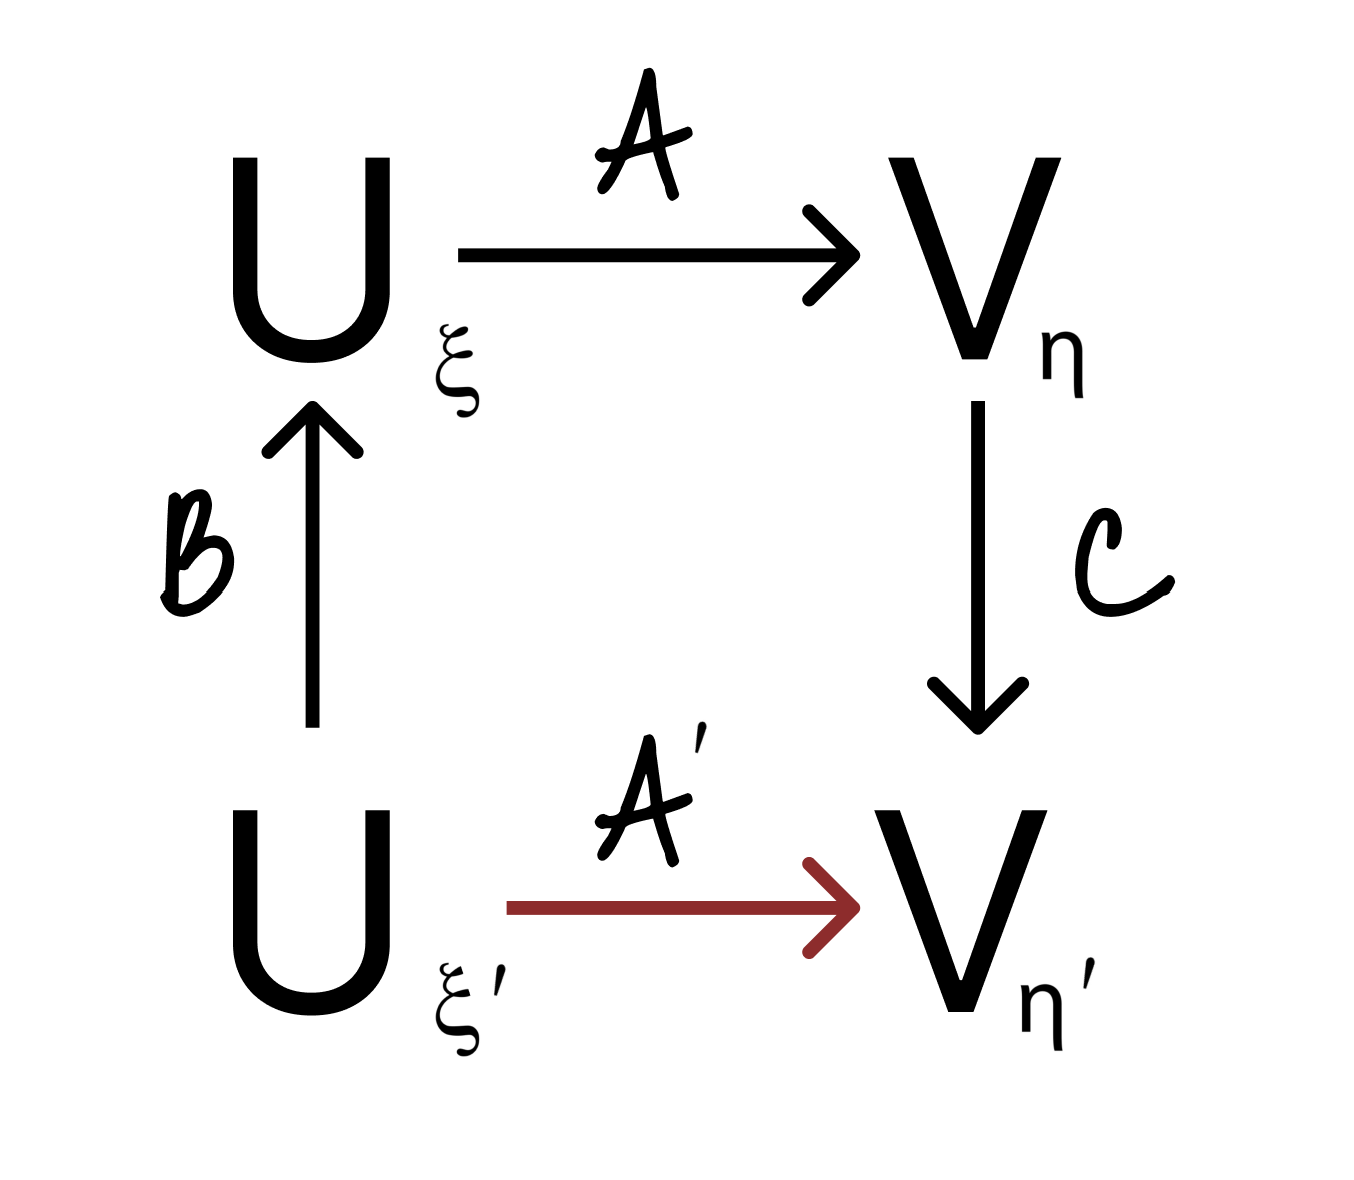
\includegraphics[width = 5cm]{assets/7_2_1.png}
\end{center}
    Воспользуемся данным рисунком, чтобы понять происходящее. Мы хотим найти матрицу $\mathcal{A}'$. Для этого, заметим, что преобразование $\mathcal{A}'$, это преобразование $\mathcal{B}$, потом примененное к нему преобразование $\mathcal{A}$, а после этого применненое к нему преобразование $\mathcal{C}$. То есть:
    $$\mathcal{A}'=\mathcal{C}\mathcal{A}\mathcal{B}$$.

    Заметим, что матрица $\mathcal{B}$, это матрица перехода из $\xi$ в $\xi'$. Это так потому что у нас просто меняется базис (про саму матрицу перехода см. одноименный раздел). Матрица $\mathcal{C}$, это $T_{\eta' \rightarrow \eta}$. Откуда, исходя из двух утверждений сверху:
    $$A' = T_{\eta' \rightarrow \eta} A T_{\xi\rightarrow \xi'}\Rightarrow A' = T^{-1}_{\eta \rightarrow \eta'} A T_{\xi\rightarrow \xi'}$$ 

\hfill Q.E.D.
%todo

\deff{Следствие:} $A \in End(V)$. $e,e'$ базисы V. $A' = T^{-1}AT$

\subsection{Инварианты линейного отображения.}

\deff{Инвариатность} называется некоторое свойство объекта, которое не меняется при определенных действиях и преобразованиях.

$A$ - линейное отображение. Ранг и дефект инварианты относительно выбора базиса.
    
